\documentclass[11pt]{article}
\usepackage{graphicx,amsmath,amsfonts,amssymb,graphicx} 
\usepackage[varg]{txfonts}
\usepackage{enumerate}
\usepackage{hyperref}
\usepackage{listings}
\usepackage{color}
\urlstyle{tt}

\usepackage{geometry}
\geometry{%
  letterpaper,
  lmargin=2cm,
  rmargin=2cm,
  tmargin=2cm,
  bmargin=2cm,
  footskip=12pt,
  headheight=12pt}
  
\usepackage{lastpage}
\usepackage{fancyhdr}
%\pagestyle{fancy}
%\headheight 35pt

\def\squarebox#1{\hbox to #1{\hfill\vbox to #1{\vfill}}}
\def\qed{\hspace*{\fill}
        \vbox{\hrule\hbox{\vrule\squarebox{.667em}\vrule}\hrule}}
\newenvironment{solution}{\begin{trivlist}\item[]{\bf Solution:}}
                      {\textbf{//} \end{trivlist}}
\lstset{
	language=MATLAB,              % choose the language of the code ("language=Verilog" is popular as well)
   tabsize=3,							  % sets the size of the tabs in spaces (1 Tab is replaced with 3 spaces)
	basicstyle=\tiny,               % the size of the fonts that are used for the code
	numbers=left,                   % where to put the line-numbers
	numberstyle=\tiny,              % the size of the fonts that are used for the line-numbers
	stepnumber=2,                   % the step between two line-numbers. If it's 1 each line will be numbered
	numbersep=5pt,                  % how far the line-numbers are from the code
	%backgroundcolor=\color{mygrey}, % choose the background color. You must add \usepackage{color}
	%showspaces=false,              % show spaces adding particular underscores
	%showstringspaces=false,        % underline spaces within strings
	%showtabs=false,                % show tabs within strings adding particular underscores
	frame=single,	                 % adds a frame around the code
	tabsize=3,	                    % sets default tabsize to 2 spaces
	captionpos=b,                   % sets the caption-position to bottom
	breaklines=true,                % sets automatic line breaking
	breakatwhitespace=false,        % sets if automatic breaks should only happen at whitespace
	%escapeinside={\%*}{*)},        % if you want to add a comment within your code
	%commentstyle=\color{BrickRed}   % sets the comment style
}                    
\begin{document}

\title{\bf{CSE397: Assignment \#4}}
\author{Nicholas Malaya \\ Department of Mechanical Engineering \\
Institute for Computational Engineering and Sciences \\ University of
Texas at Austin} \date{} 
\maketitle
\newpage

\subsection*{ Problem 1}
\textbf{Frequency-domain inverse wave problem.} 

\begin{enumerate}
\item[(a)]
\begin{solution}
The weak form of the state equation is given by: 
\begin{displaymath}
\int_{\Omega}\nabla u \cdot \nabla p - k^2mup - fp\hspace{2 mm}dx -
 \int_{\Gamma}p\nabla u \cdot n\hspace{2 mm}ds \hspace{1 cm} \forall p
 \in H^1_0(\Omega) 
\end{displaymath}
However since p = 0 on the boundary then the boundary term is zero. The
 Lagragian is therefore:  
\begin{displaymath}
\mathcal{L}(u,p,m) := \int_{\Omega}\nabla u \cdot \nabla p - k^2mup -
 fp\hspace{2 mm}dx + \int_{\Omega}\left(u - u^{obs}\right)^2 dx +
 \frac{\beta}{2}\int_{\Omega}\nabla m \cdot \nabla m dx 
\end{displaymath}
We now take variations with respect to each of the parameters:
\begin{align}
\delta_u\mathcal{L}(\tilde{u}) &= \int_{\Omega}(u-u^{obs})\tilde{u} +
 \nabla\tilde{u}\cdot\nabla p - k^2m\tilde{u}p \hspace{2 mm} dx = 0
 \hspace{1 cm} \forall\tilde{u} \in H^1_0(\Omega) \nonumber \\ 
\delta_p\mathcal{L}(\tilde{p}) &= \int_{\Omega} \nabla u \cdot
 \nabla\tilde{p} - k^2mu\tilde{p} - f\tilde{p} \hspace{2 mm} dx = 0
 \hspace{1 cm} \forall\tilde{p} \in H^1_0(\Omega) \nonumber \\ 
\delta_m\mathcal{L}(\tilde{m}) &= \int_{\Omega} \beta \nabla m \cdot
 \nabla\tilde{m} - k^2\tilde{m}up \hspace{2 mm} dx = 0 \nonumber 
\end{align}
The last of these equations is the gradient equation. It depends
 on both p and u which come from the adjoint and state
 equations. u is found to be the solution of the
 following: 
\begin{align}
-\Delta u - k^2mu &= f\hspace{5 mm} \text{on } \Omega \nonumber \\
u &= 0 \hspace{5 mm} \text{on } \partial\Omega \nonumber
\end{align}
and $p$ is found to be the soultion to the adjoint equation:
\begin{align}
-\Delta p - k^2mp &= u^{obs} - u \hspace{5 mm} \text{on } \Omega \nonumber \\
p &= 0 \hspace{5 mm} \text{on } \partial\Omega \nonumber.
\end{align}
Using the solutions of these equations then gives the gradient with
 $\delta_m\mathcal{L}(\tilde{m}) = 0$. 
\end{solution}

\item[(b)] Derive an expression for the (infinite dimensional) action of
	   the Hessian in a direction m in the single source and frequency case.

\begin{solution}
To get the application of a Hessian on a vector, one needs the second
 variation of the three weak forms in the previous section. These are: 
\begin{align}
\left(\delta_u+\delta_m+\delta_p\right)\left(\delta_u\mathcal{L}\right)
 &= \int_\Omega \hat{u}\tilde{u} - k^2\hat{m}\tilde{u}p -
 k^2m\tilde{u}\hat{p} + \nabla\tilde{u}\cdot\nabla\hat{p} \hspace{2 mm}
 dx \nonumber \\ 
\left(\delta_u+\delta_m+\delta_p\right)\left(\delta_p\mathcal{L}\right)
 &= \int_\Omega \nabla\hat{u}\cdot\nabla\tilde{p} - k^2m\hat{u}\tilde{p}
 - k^2\hat{m}u\tilde{p} \hspace{2 mm} dx \nonumber \\ 
\left(\delta_u+\delta_m+\delta_p\right)\left(\delta_m\mathcal{L}\right)
 &= \int_\Omega \beta\nabla\hat{m}\cdot\nabla\tilde{m} -
 k^2\tilde{m}\hat{u}p - k^2\tilde{m}u\hat{p} \hspace{2 mm} dx \nonumber 
\end{align}
However this introduces two new variables $\hat{p}$ and $\hat{u}$
 which need to be solved for. From the second variation one gets
 $\hat{u}$. Its strong form is given by:  
\begin{align}
-\Delta\hat{u}-k^2m\hat{u} &= k^2\hat{m}u \hspace{5 mm} \text{on }
 \Omega \nonumber \\ 
\hat{u} &= 0 \hspace{5 mm} \text{on } \partial\Omega \nonumber
\end{align}
Similarly $\hat{p}$ is given by the solution to the second variation of the adjoint equation:
\begin{align}
-\Delta\hat{p} - k^2m\hat{p} &= k^2\hat{m}p - \hat{u}\hspace{5 mm} \text{on } \Omega \nonumber \\
\hat{p} &= 0 \hspace{5 mm} \text{on } \partial\Omega \nonumber
\end{align}
Using the solution to the state equation ($u$), the solution to the
 adjoint equation ($p$), $m$, the solution to the second variation of
 the state equation ($\hat{u}$), the solution to the second variation of
 the adjoint equation ($\hat{p}$), and given a direction $\hat{m}$, the
 action of the Hessian in a direction $\hat{m}$ is given by: 
\begin{displaymath}
\int_\Omega \beta\nabla\hat{m}\cdot\nabla\tilde{m} -
 k^2\tilde{m}\hat{u}p - k^2\tilde{m}u\hat{p} \hspace{2 mm} dx = 0 
\end{displaymath}
\end{solution}

\item[(c)] Derive an expression for the (infinite dimensional) gradient
	   for an arbitrary number of sources and frequencies. How many
	   state and adjoint equations have to be solved for a single
	   gradient computation? 

\begin{solution}
The gradient is still calculated in the same manner as in the previous
 case with a single source and frequency. Therefore it is the variation
 of the Lagrangian with respect to m. However, now for each $u_{ij}$
 there is a corresponding adjoint variable $p_{ij}$ and the Lagrangian
 takes a slightly different form than before. With all of the
 frequencies and sources the minimization problem is given as stated: 
\begin{displaymath}
\min_m J(m) :=
 \frac{1}{2}\sum_{i=1}^{N_f}\sum_{j=1}^{N_s}\int_{\Omega}\left(u_{ij} -
 u_{ij}^{obs}\right)^2 dx + \frac{\beta}{2}\int_{\Omega}\nabla m \cdot
 \nabla m dx 
\end{displaymath}
To form the Lagrangian this needs to be paired with the state equation. However the state equation for a single $u_{ij}$ is given by:
\begin{align}
-\Delta u_{ij} - k_i^2m(x)u_{ij}(x) &= f_j(x)\hspace{5 mm} \text{on }
 \Omega \hspace{5 mm} i = 1, 2, ..., N_f \hspace{5 mm} j = 1, 2, ...,
 N_s \nonumber \\ 
u_{ij} &= 0 \hspace{5 mm} \text{on } \partial\Omega \nonumber
\end{align}
Therefore one needs to carry all $N_sN_f$ of these into the
 Lagrangian. Note that in weak form, a single state equation looks like: 
\begin{displaymath} 
\int_{\Omega}\nabla u_{ij} \cdot \nabla p_{ij} - k_i^2mu_{ij}p_{ij} -
 f_jp_{ij}\hspace{2 mm}dx \hspace{1 cm} \forall p_{ij} \in H^1_0(\Omega) 
\end{displaymath}
Again the boundary term is zero since $p_{ij} = 0$ on the boundary. With
 the weak forms for each of the $u_{ij}$, the Lagrangian is given by: 
\begin{displaymath}
\mathcal{L} := \sum_{i=1}^{N_f}\sum_{j=1}^{N_s}\int_{\Omega}\left(\nabla
 u_{ij} \cdot \nabla p_{ij} - k_i^2mu_{ij}p_{ij} - f_jp_{ij}\right)dx +
 \frac{1}{2}\sum_{i=1}^{N_f}\sum_{j=1}^{N_s}\int_{\Omega}\left(u_{ij} -
 u_{ij}^{obs}\right)^2 dx + \frac{\beta}{2}\int_{\Omega}(\nabla m \cdot
 \nabla m) dx 
\end{displaymath}
Taking a variation with respect to $m$ of this gives:
\begin{displaymath} 
\int_{\Omega} \beta (\nabla m \cdot \nabla\tilde{m})dx -
 \sum_{i=1}^{N_f}\sum_{j=1}^{N_s}\int_{\Omega}(k_i^2\tilde{m}u_{ij}p_{ij})dx 
\end{displaymath}
This will give the gradient for a point $m$, provided a solution is
 available for each of the $u_{ij}$ and the $p_{ij}$. Obtaining those
 solutions requires $N_sN_f$ solves of the state and adjoint equations
 for a total of $2N_sN_f$ PDE solves. 
\end{solution}
\end{enumerate}

\newpage
\subsection*{Problem 2}

\begin{enumerate}
\item[(a)] Report the solution of the inverse problem and the number of
	  required iterations for the following cases:


%Report the reconstructions and the number of required
%	  iterations for the following cases:

\begin{enumerate}
 \item[$\bullet$] Noise level of 0.01 (roughly $1\%$ noise), and
	      regularization $\beta = 5 \cdot 10^{-10}$.
 \item[$\bullet$] Same, but with $\beta = 0$, i.e., no regularization. 
 \item[$\bullet$] No noise, and use $m \equiv 4$ and $m \equiv 8$ as
	      initial guesses for the parameter. Do you find the same
	      solution? Explain the behavior.  
\end{enumerate}
\begin{solution}
The following table summarizes the number of iterations for each of the
 desired start conditions: 
\begin{center}
\begin{tabular}{| c | c | c | c |} \cline{1-4}
Noise & $\beta$ & $m$ & No. of Iterations \\ \cline{1-4}
0.01 & 5E-10 & 8 & 284 \\ \cline{1-4}
0.01 & 0.0 & 8 & 27 \\ \cline{1-4}
0.0 & 0.0 & 8 & 27 \\ \cline{1-4}
0.0 & 0.0 & 4 & 24 \\ \cline{1-4} 
\end{tabular} 
\end{center}
The results of these trials are can be quite different. The case with noise
 and regularization yields the following result: 
\begin{center}
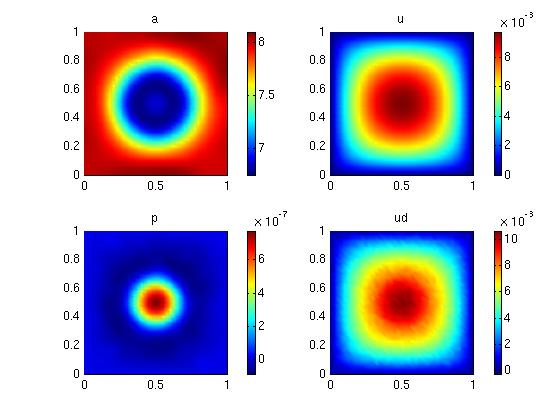
\includegraphics[width = 6 cm]{figs/prob2aNoiseRegM8.jpg}
\end{center}

The case with no regularization resulted in:
\begin{center}
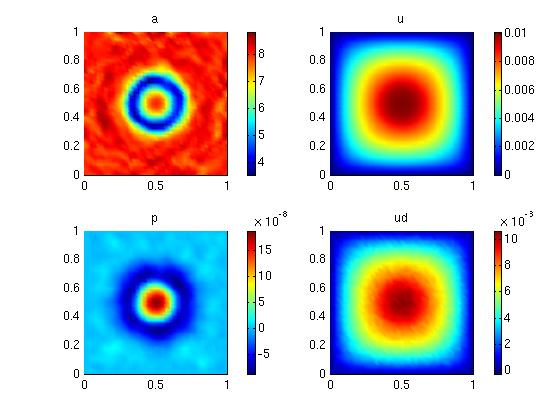
\includegraphics[width = 6 cm]{figs/prob2aNoiseNoRegM8.jpg}
\end{center}

The case with no noise and no regularization and $m = 8$:
\begin{center}
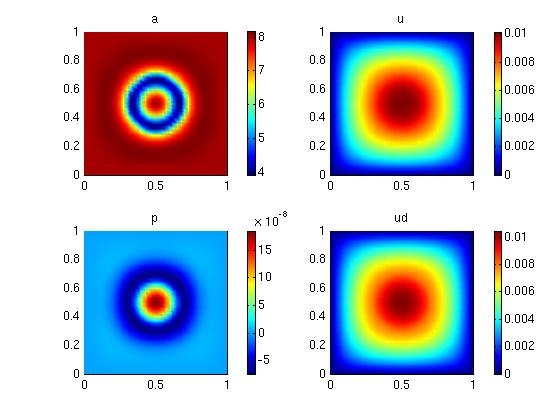
\includegraphics[width = 6 cm]{figs/prob2aNoNoiseNoRegM8.jpg}
\end{center}

The case with no noise and no regularization and $m = 4$:
\begin{center}
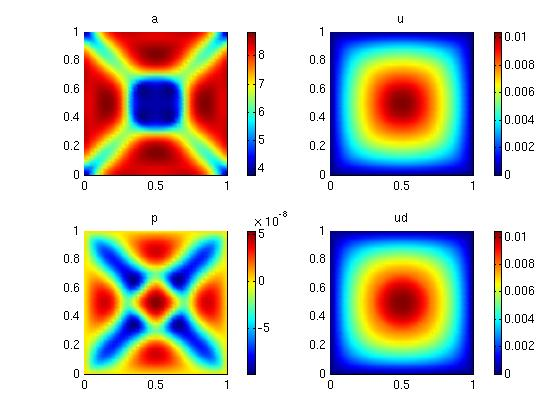
\includegraphics[width = 6 cm]{figs/prob2aNoNoiseNoRegM4.jpg}
\end{center}

Note the difference in the final cases where the result for $m = 4$ ($a$
 in the image) is vastly different from the other results. This is a
 direct result of steepest descent being dependent on the start
 value. The case with no noise or regularization with $m = 8$ provides a 
 solution close to the truth. Similarly
 the $m = 4$ solution is close to the true solution except for the
 diagonals. Note also that the $p$ values are also rather
 different. This is likely due to the adjoint being sensitive to
 $m$. $u$ should also be sensitive to $m$, but the end result look
 roughly the same because of the misfit penalization.
\end{solution}

\item[(b)] Add the advective term v = (30, 0) to the inverse problem and its COMSOL
	  implementation and plot the resulting reconstruction of m for
	  a noise level of 0.01 and for a reasonably chosen regularization parameter.

\begin{solution}
After adding the advective term, the result for a noise level of 0.01
 and regularization of 5e-10 is given by: 
\begin{center}
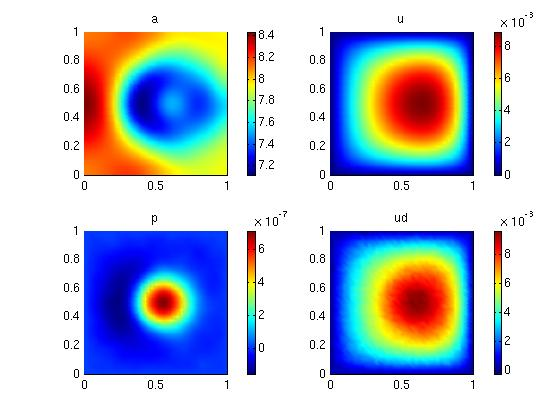
\includegraphics[width = 6 cm]{figs/prob2bNoiseRegM8.jpg}
\end{center}
\end{solution}

\item[(c)] Since the coefficient m is discontinuous, a better choice of
	   regularization is total variation
	   rather than Tikhonov regularization, to prevent an overly smooth
	   reconstruction. Modify the implementation and plot the result
	   for a reasonably chosen regularization parameter


%Since the coefficient $m$ is discontinuous, a better choice is to use total variation
%regularization rather than Tikhonov regularization to prevent an overly smooth
%reconstruction. Modify the implementation and plot the result for a reasonably
%chosen regularization parameter.

\begin{solution}
 Since one is switching to a total variational regularization parameter,
 now two choices of parameters are needed. For the solution shown below,
 the calculation was done with the same advective term, regularization
 parameter beta, and noise level as before in part b, however it also
 uses a tau of 1e-1 as requested. The result found is: 
\begin{center}
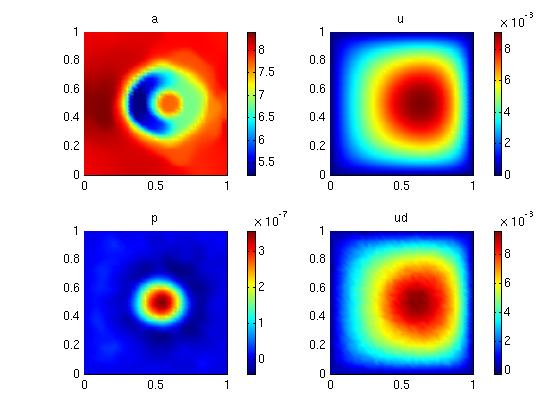
\includegraphics[width = 6 cm]{figs/prob2c.jpg}
\end{center}
Note that the drift from the advective term is not fully removed by this
 regularization, though the solution is much closer than with Tikhonov
 regularization. 
\end{solution}
\end{enumerate}

\newpage
\subsection*{Code}
Here is the code for part c:
\lstinputlisting{code/elliptic_sd_ip_adv_TV.m}
\end{document}